\documentclass[10pt,twoside,a4paper]{article}

\usepackage{fancyhdr}

\usepackage{lastpage}       % ``n of m'' page numbering
\usepackage{lscape}         % Makes landscape easier

\usepackage{verbatim}       % Verbatim blocks
\usepackage{listings}       % Source code listings
\usepackage{epsfig}         % Embed encapsulated postscript
\usepackage{array}          % Array environment
\usepackage{array}          % Array environment
\usepackage{enumitem}       % Required by Tom Johnson's exam question header

\usepackage{hhline}         % Horizontal lines in tables
\usepackage{siunitx}        % Correct spacing of units
\usepackage{amsmath}        % American Mathematical Society
\usepackage{amssymb}        % Maths symbols
\usepackage{amsthm}         % Theorems

\usepackage{ifthen}         % Conditional processing in tex

\usepackage[skip=0.5cm]{parskip}

\usepackage[top=3cm,
            bottom=3cm,
            inner=2cm,
            outer=2cm]{geometry}

% If you have any additional \usepackage commands, or other
% macros or directives, put them here.  Remember not to edit
% files in the template directory because any changes will
% be overwritten when template updates are issued.
\usepackage{float,graphicx}
\usepackage{amsmath}
\usepackage{amssymb}
\usepackage{caption}
\usepackage{subcaption}

\usepackage[absolute,overlay]{textpos}

\newcolumntype{C}{>$c<$}
\graphicspath{ {./images/} }

\newcommand{\notimplies}{%
  \mathrel{{\ooalign{\hidewidth$\not\phantom{=}$\hidewidth\cr$\implies$}}}}
\newcommand{\Mod}[1]{\ (\mathrm{mod}\ #1)}
\newcommand{\Z}{\mathbb{Z}}
\newcommand{\R}{\mathbb{R}}
\newcommand{\Q}{\mathbb{Q}}
\newcommand{\N}{\mathbb{N}}


\title{Delay-Tolerant Link-State Routing}
\author{Ben Andrew, ba405\\Magdalene College}
\date{\today}


\begin{document}
\maketitle


\section{Declaration of Originality}

The project contains 4605 lines of code, consisting of 3944 lines of C and 661 lines of Python

\section{Proforma}

\section{Table of Contents}

\section{Introduction}

This project aims to evaluate delay-tolerant modifications made to a link-state routing protocol for network environments with low reliability. It is motivated by similar conditions being seen in network infrastructure in remote developing regions, where issues such as unreliable power can cause a severe drop in packet delivery. We see how modifications made to the routing protocol can reduce this.

\subsection{Background}

One problem in a network is how to route packets from one node to another, on a path through the network hopping from node to node. A routing protocol describes how routers communicate with each other to distribute information about the topology of the network in order for each router to choose optimal routes to other nodes, and thus make optimal local forwarding decisions for incoming packets. One class of routing algorithms called link-state protocols aim for every router in the network to have a full view of the network topology, so when a change occurs in the network (e.g. a link fails), that information is propagated outwards from router to router, with the change being incorporated into each router's internal representation of the network.

Traditional routing protocols such as OSPF treat failures as final, making the assumption that the failed link will not come back up anytime soon. If alternate routes exist they route around the failure to maintain connectivity as much as possible. However if no alternate routes exist (i.e. the network has been partitioned) then no data can be sent at all, and all packets sent after the failure will be dropped.

However in environments such as developing regions with unreliable network infrastructure, partitions due to temporary link failures are a common occurrence. In this case the performance of traditional routing protocols can drop dramatically, in some cases preventing any end-to-end communication entirely. The routing protocols used in these situations must be designed to compensate for these failures in order to provide good service.

One approach to make traditional routing more `delay-tolerant' is by allowing routing paths to be advertised through down links, and to use a `store-and-forward' mechanism for packet forwarding where if the link on the outgoing interface is down, any packets incoming to the router that would be forwarded out on that interface are buffered in-memory by the router. When the link comes back up, all of the buffered packets are sent out of the desired interface. This maintains end-to-end connectivity as much as possible and decreases the drop rate of packets dramatically.

\begin{figure}[H]
\centering
\begin{subfigure}{.45\textwidth}
  \centering
  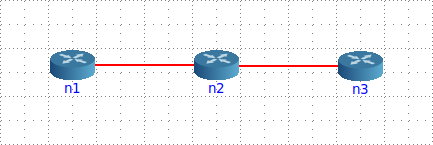
\includegraphics[width=1\linewidth]{pathalogical_topology}
  \label{fig:pathalogical_topology}
\end{subfigure}%
\begin{subfigure}{.55\textwidth}
  \centering
  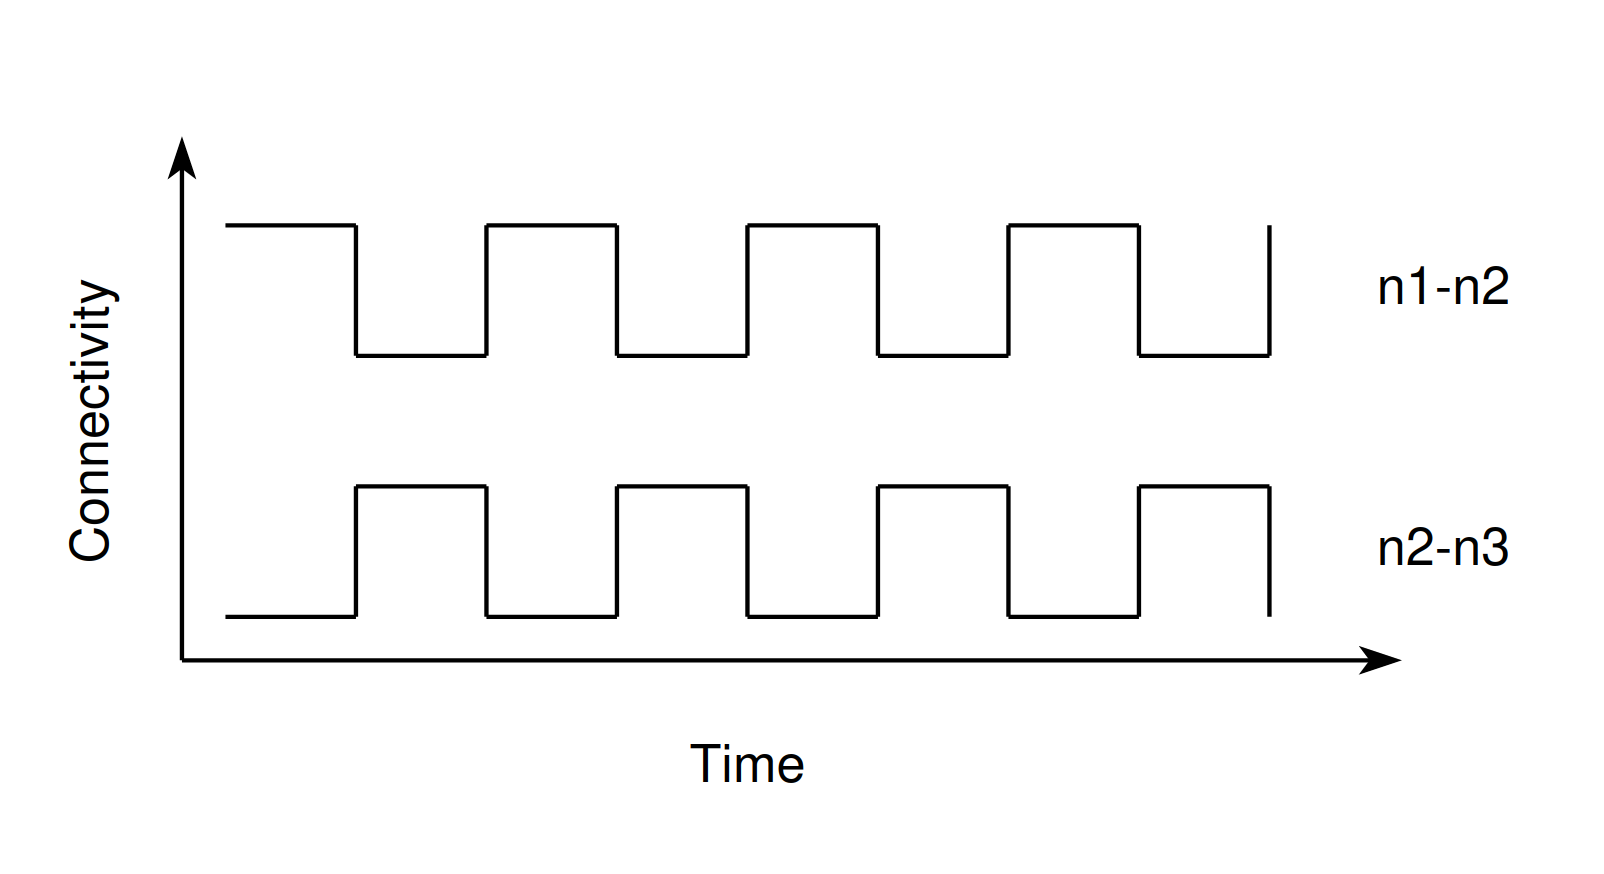
\includegraphics[width=1\linewidth]{pathalogical_graph}
  \label{fig:pathalogical_graph}
\end{subfigure}
\caption{Pathalogical case where a store-and-forward technique allows packets to be delivered despite no end-to-end connection. Traditional techniques will drop all packets.}
\label{fig:pathalogical}
\end{figure}

\subsection{Objectives of the Project}

The primary goal of this project is to compare the performance of a protocol using traditional link-state routing with a modified version implementing delay-tolerant features. To have control over the behaviour of the protocols both are implemented from scratch in C, with the design based off of the OSPF protocol. The evaluation will focus mainly on the drop rate of packets, as well as the delay of packet arrivals. We do the evaluation by running the protocols on an industry-grade network emulator that provides a realistic testing environment with full control over the network properties.

\subsection{Related Work}

There has been much research into `mobile ad-hoc networks', where mobile nodes physically move around and have intermittent and unpredictable connectivity with other nodes. This requires a dramatic change in network protocol design, but for our situation it is not necessary. Link failures in a mobile network are usually due to topology changes, but networks in developing regions have largely static topologies with modem or satellite links, where link failures - mostly due to congestion or unreliable power - do not imply that the topology has changed. When the failure is resolved the topology will be the same as before, thus we are able to use a well-understood link-state paradigm with comparatively minor modifications, making deployment far easier and minimising wasted resources from unnecessary features.



\section{Preparation}

\section{Implementation}

\subsection{Repository Overview}

\begin{verbatim}
dtlsr                        Root
|- configs                   CORE config files
|- include                   Include directory
|  |- algorithm
|  |- network
|  '- process
|- src                       Source directory
|  |- algorithm
|  |- network
|  '- process
|- tests                     Unit tests directory
|  |- algorithm
|  |- network
|  '- process
|- tools                     Custom development tools
'- core-py                   Custom CORE scripts
\end{verbatim}

\texttt{algorithm} contains pure algorithms and data structures, for example graph, graph searching, and heap implementations.

\texttt{network} contains functionality for socket manipulation, sending data over the network, and packet listening/replay.

\texttt{process} contains funtionality for interacting with both CORE and the Unix OS, for example retreiving node information, logging, and manipulating the Unix routing table.

The project was implemented almost entirely in C, with CORE-specific scripts in Python. I used the CMake build system and Check unit testing framework.


\subsection{CORE Background}

The Common Open Research Emulator (CORE) is a network emulator that models nodes as lightweight Unix virtual machines, complete with filesystems and network interfaces. It comes out of the US Naval Research Laboratory and was developed by Boeing Research and Technology.

\begin{minipage}{1\textwidth} \centering
	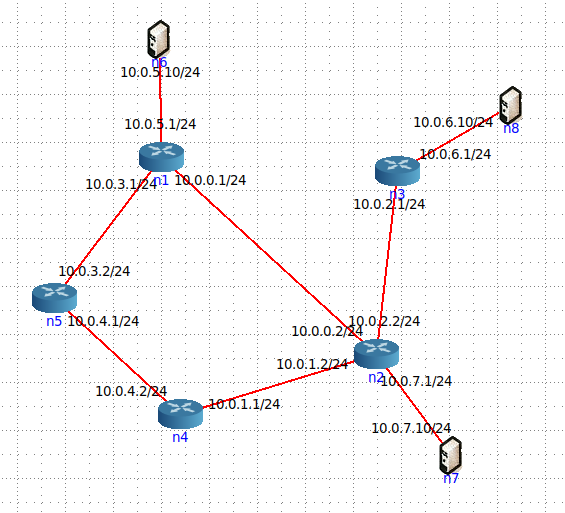
\includegraphics[width=0.6\textwidth]{core_topology}
	\captionof{figure}{Example emulated network in the CORE GUI, showing routers and hosts.}
\end{minipage}

Programs can be written for these nodes and run as Unix processes via a Python API. These processes are then able to send and receive data through the emulated network via standard Unix socket programming. The emulated routers contain default routing protocol implementations, such as OSPFv2 and v3 from the Quagga protocol suite, which can be disabled and replaced by custom implementations. As well as this, standard network testing tools like \texttt{ping} can be run on emulated endpoint hosts, making testing and evaluation of the network surprisingly simple.

Link properties can be programmatically customised through the Python API, with properties including bandwidth, delay, loss, and jitter. This will aid greatly in evaluation, for example simulating a link failure by setting the loss rate of a node to 100\%, allowing us to create network partitions.

One limitation is that CORE operates in real-time using the OS's clock, and thus the performance of the simulated network is somewhat dependent on the performance of the machine it's being run on. I will therefore be taking great care to create a reliable and statistically sound testing environment, for example setting processor priority, not running other programs, and taking baseline measurements to compare against.

The sharing of the clock has the advantage that when deriving the time between events on different virtual machines we don't need to account for any clock drift; the time difference will be as exact as if they were the same machine. This will make evaluation easier and more accurate, reducing the error.

\subsection{Link-State Routing Design}

The link-state routing protocol that I implemented is split into two programs, \texttt{heartbeat} and \texttt{lsr}. Routers run both programs, and hosts run only \texttt{heartbeat}.

\texttt{heartbeat} sends periodic heartbeat messages to all neighbouring nodes, notifying them that the connecting link is still up. The message is received by \texttt{lsr}. Hosts run \texttt{heartbeat} to notify their gateway router of their existence, so that the router can advertise the corresponding route.

\texttt{lsr} implements the bulk of the protocol. It maintains the link-state graph representation of the network, manipulates the node's routing table, and sends link-state announcements (LSAs) in response to detected changes in the network.

These changes are detected in one of three ways. When we state a link is UP or DOWN we mean the router's link-state representation of the network:
\begin{enumerate}
	\item
	A heartbeat message is received from a neighbour with a DOWN link. We set the link to be UP.
	
	\item
	A heartbeat is not received in time from a neighbour with an UP link. We set the link to be DOWN.
	
	\item
	An LSA is received from a neighbour. If they have any information more recent that ours that causes a change to our network representation when merged in, a change is detected.
\end{enumerate}

Both programs lend themselves to an event-driven design, and so I used file descriptors multiplexed with the \texttt{select} Unix system call to detect and respond to events. The \texttt{select} call blocks the process from running until one of the specified file descriptors is ready to be used, at which point the OS gives the process back control along with information about which file descriptor is ready. Using this we can implement a coarse event system. As examples, receiving socket file descriptors trigger as `ready' when data has arrived and is ready to be read, and timer file descriptors trigger as `ready' when the timer has expired. One can see how these can be composed to create a responsive distributed protocol that uses system resources efficiently, rather than just spinning waiting for something to happen.

Heartbeats and LSAs are recieved on sockets with distinct ports, allowing them to be differentiated easily by the Unix socket API at the UDP layer. While these are purely link-level communications and as such do not require UDP or even IP information, the socket API is an easy abstraction to use and allows me to reuse code from other parts of the codebase, minimising the possibility of introducing bugs.

A heartbeat message is a UDP packet with only header, no payload. An LSA is a UDP packet whose payload is the sending node's graph representation of the network, simply copied into the payload using \texttt{memcpy}. The graph representation uses statically sized arrays rather than dynamically sized `\texttt{malloc}ed' ones, to make allocation and indexing simpler. While it would be more space-efficient to pack the graph into a more compressed structure for sending over the link, the network topologies that I use in the evaluation are not large enough for this to be an issue. It would be a simple fix if this became an issue.

We send LSAs to our neighbours whenever we detect a change in the network (as specified above). This means we propagate link-state information as quickly as possible, minimising convergence time. We also send only when we detect changes with respect to our knowledge of the network so that we don't cause infinite looping of updates.

\subsubsection{Local and Global Link-State}

We have two levels of representation for our network representation: a minimal global representation of the entire network and a detailed representation of the immediate neighbourhood of the local node.

For each node in the global graph, we store for each link information like the source IP, neighbour destination IP, the status of the link, the derived metric associated with the link, and a timestamp specifying how old our knowledge of that link is, for merging purposes.

The local graph consists solely of our node along with more in-depth information about links connecting us to our immediate neighbours. Along with all of the information contained in a global node, we also have for each link a timer for timing out heartbeats and the interface which that link goes out on. We take the locally-derived information and feed it into the global graph, which then gets shared with the rest of the network via LSAs.

\subsubsection{Route Generation}

Routes are derived from the link-state graph, where we compute the shortest path from ourselves to every other node in the graph using Dijkstra's algorithm. The metric for a path is given as the number of hops in the path, which I chose over a more standard OSPF-style metric depending on bandwidth as I am more concerned with delay than throughput. Notably, if a link is though to be DOWN, we disallow the pathfinding to go through that link.

After pathfinding we have for each destination address a `next-hop' address. We first generalise each specific destination address to its 24 bit subnet, zeroing out the last 8 bits. Many of these routes can then be merged together, for example if two destinations are part of a single subnet and have the same next-hop. This route aggregation reduces the size of the routing table.

We keep track of which routes we have previously added to the routing table, and mark off those that we have regenerated from the updated graph. If we have previously added routes that are not marked off, then we know that route no longer exists and we can remove it from the routing table. This may happen if a link goes down or a better alternative route appears.

With invalid routes removed, we can then add all of our new routes to the routing table. Manipulation of the Unix routing table is done through the \texttt{ioctl}, a system call for interacting with OS devices through a file descriptor interface. We pass a flag corresponding to route addition or deletion, along with a `\texttt{route}' struct containing the route details.

\subsection{Delay-Tolerant Modifications}

For the delay-tolerant version of the protocol suite, we replace the \texttt{lsr} executable with \texttt{dtlsr}, keeping \texttt{heartbeat} the same. \texttt{dtlsr} uses mostly the same source files as \texttt{lsr}, with the delay-tolerant modifications enabled by \texttt{\#ifdef DTLSR} preprocessor switches. \texttt{dtlsr} maintains many of the same implementation design decisions as above with a few additions.

Firstly, in the pathfinding algorithm we allow paths to be generated through DOWN links so that when we update the routing table packets will be sent along the path up to the DOWN link, and buffered there until the link comes back up. The metric is modified to be, instead of hop count, an exponential time-average of the uptime history of all links along the path, so that nodes along unreliable paths will have a much higher cost. These uptime histories are maintained locally for neighbour links only; when we advertise our link state using LSAs we share only the derived metric. The metric for a path is still the summation of costs of each link along the path, which is a natural way to combine delay-dependent metrics.

An interesting edge case is when a link goes down connecting a host with its gateway router. As the host runs \texttt{heartbeat} the router will be aware that the link is down and will buffer any traffic coming in along the advertised route with the host as the destination. However any traffic the host wants to send outwards will not be buffered by itself as it is not running any `delay-tolerant' routing software; the host will have to deal with retransmissions as it will not buffer any data locally. We could theoretically develop a minimal version of the protocol that runs on hosts and only does buffering to solve this issue.

\subsubsection{Packet Buffering}

When a link is DOWN, in our delay-tolerant context we may still advertise routes going through it as if it was open, and so we may have traffic routed through us expecting to move through the link. Thus we must buffer this traffic locally until either the link comes back up or a better alternative route appears, at which point we send it on.

We use the \texttt{tcpdump} tool for interface listening. When a router knows a connected link is down, it starts listening on all interfaces and dumping received packets to a \texttt{pcap} file, according to a packet filter that only dumps packets going to an IP address that we route to via the down interface. \texttt{tcpdump} is interacted with via the \texttt{libpcap} C library linked in statically with the executable, with the packet filter programmed using the Berkeley Packet Filter (BPF) language. An important optimisation is to place this \texttt{pcap} file on a RAM disk to maximise throughput and minimise latency that can occur when storing files on an SSD or even a HDD.

When the link comes back up, we stop listening for packets and dumping them to the file, and close the file. From now incoming packets are being routed out of the interface correctly so we don't want to duplicate data by buffering then resending it. We make use of a command-line tool, \texttt{tcpreplay}, which allows packets from \texttt{pcap} files to be replayed out of  an interface. We do this, and then delete the file. Described here is the case of a single failing link, but when multiple links are concurrently failing and coming back up we of course need to be more careful about listening for and replaying only the right data.

I chose to use existing tools for packet buffering due to the complexity of this problem, as well as issues with reliability. Even a mature and tested tool like \texttt{tcpdump} still cannot catch all incoming packets at higher speeds, I would have no hope of implementing a suitable alternative in the time I had; it would likely be a part II project in its own right.

\subsection{Implementation Practicalities}

Some parts of the implementation were hard-coded or have inefficient solutions to aid in creating a functional piece of software that could be evaluated more quickly. These are sections that have no impact on the evaluation of the protocol as a solution to the routing problem, or are even completely unrelated to routing in general.

As an example I ran into the issue of `neighbour discovery', where nodes generally use ARP to discover the existence of neighbouring nodes on their interfaces. The ARP table in CORE proved unreliable, and as this is a link-layer problem unrelated to routing I simply hardcoded all immediate neighbours in configuration files. Implementing actual neighbour discovery would provide no practical benefits to the evaluation, and could even negatively impact it if my implementation was unreliable or had varying performance.

An example of hardcoding is that the memory representation of the link-state graph is statically allocated, i.e. the maximum number of nodes in the network is specified as a compile-time constant. The advantage of this is that it makes indexing and bounds checking very easy and computationally efficient, however we have the twin disadvantages of wasting memory if we are below the maximum number of nodes, and much worse, crashing if the number of nodes increases beyond the maximum. However for the evaluation this is not an issue, as I know beforehand the size and topology of all networks being tested, and can adapt the compile-time maximum as needed. If used in a real network, the memory representation would have to be changed to allow dynamic sizing.

While CORE supports IPv6 addressing, I restricted myself to only supporting IPv4 to reduce the unnecessary complexity of supporting another addressing scheme that would have no impact on the performance of the routing protocol, and thus not help my evaluation at all.


\section{Evaluation}

The evaluation is done using the CORE emulator. We define a network topology of hosts and routers, with the routers running either the LSR or DTLSR routing protocol, in order to compare the performance of both for a variety of metrics on a variety of different topologies.

We first determine the convergence behaviour of the protocols, to provide a baseline of the testing environment. This is done with LSR, but as DTLSR's system for this is identical the results are valid for both.

We then do a full comparison of the delay of packet arrivals in LSR and DTLSR in a number of topologies, importantly providing the overall packet loss percentage as well.

\subsection{Convergence}

The convergence time of the link-state protocol, is the time between the state of the graph updating (e.g. a link going down), and that change being detected and incorporated into the routing table of a particular node in the network. As changes are propagated from node-to-node, we expect that convergence time increases as we look at nodes further from the changing link. We will distinguish the convergence time in response to links going down, and links coming back up, as these are detected in different ways. 

\begin{minipage}{1\textwidth} \centering
	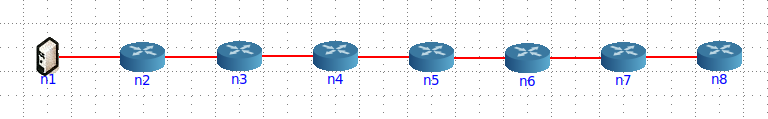
\includegraphics[width=0.7\textwidth]{conv_topology}
	\captionof{figure}{`Convergence' network topology. We flap link \texttt{n1-n2}}
	\label{fig:conv_topology}
\end{minipage}

Our testing topology is a long chain of routers, with the flapping link at one end and the update messages being propagated down the chain. This gives us a way to detect how long it takes a node to detect the change for each number of router `hops'. We consider the zero-hop node \texttt{n2} to be that directly attached to the flapping link.

We flap the link using the Python scripting API that CORE provides, waiting 4 seconds between each state change - long enough that we guarantee that all nodes have fully converged before we modify the state again. We log the time when this occurs.

We monitor each node's routing table using the \texttt{route} Unix utility, with a simple Python script that logs the time when we detect that the route corresponding to node \texttt{n1} has either appeared or disappeared from the table, respective to the link being up or down. We can then analyse the data to determine the time between the link changing state, and each node detecting this change and modifying its routing table accordingly.



\begin{figure}[H]
\centering
\begin{subfigure}{.5\textwidth}
  \centering
  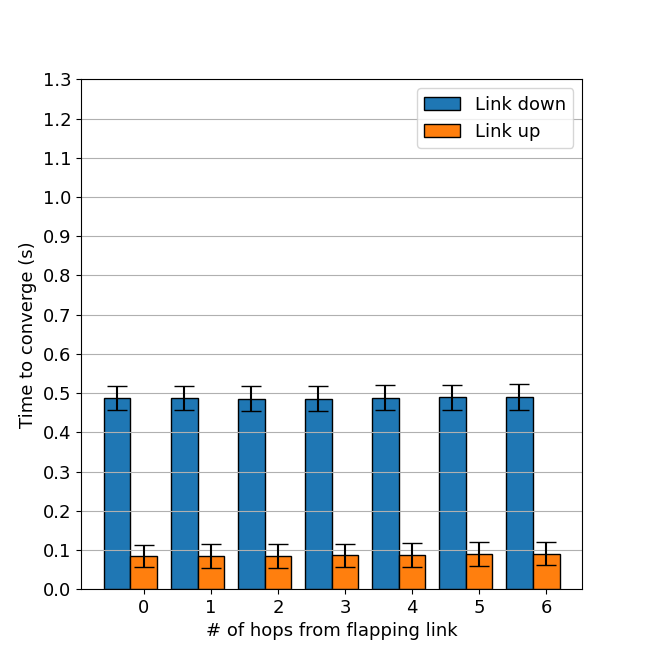
\includegraphics[width=1\linewidth]{conv_1ms}
  \caption{Link delay of \SI{1}{\ms}}
  \label{fig:conv_1ms}
\end{subfigure}%
\begin{subfigure}{.5\textwidth}
  \centering
  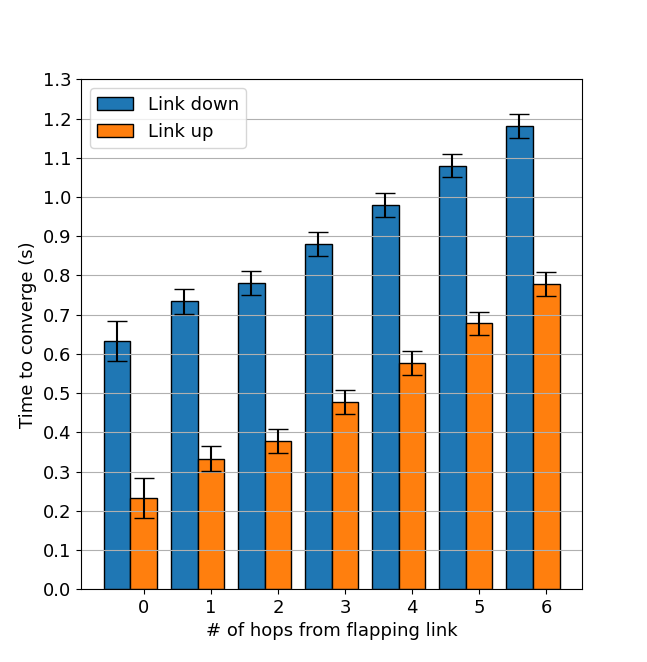
\includegraphics[width=1\linewidth]{conv_100ms}
  \caption{Link delay of \SI{100}{\ms}}
  \label{fig:conv_100ms}
\end{subfigure}
\caption{Protocol convergence times, for both the link going down, and the link coming back up. Error bars are the interquartile range.}
\label{fig:conv}
\end{figure}

We do convergence testing with link delays of \SI{1}{\ms} and \SI{100}{\ms}. A link delay of \SI{100}{\ms} is large enough to verify that the convergence time depends on the hop count, from the propagation time, while a delay of \SI{1}{\ms} is what we use for the rest of the evaluation, so it is useful to include as a baseline.

In \ref{fig:conv_1ms} we see that the zero-hop node \texttt{n2} has a `convergence' time greatly less than the rest of the nodes, which is because \texttt{n2} detects the change using the link-layer heartbeat section of the protocol. For the link being down our detection depends on a heartbeat timeout after not receiving a heartbeat. For being up our detection depends on receiving a heartbeat from our neighbour. We justify the time difference between up and down with the fact that the heartbeat timeout must necessarily be longer than the heartbeat sending period.

Hop counts of 1 and above rely on the network-layer section of the protocol, with link-state information being sent from node to node. As LSAs are propagated as soon as they are received, we are bounded mainly by the link delay, which we can see in the difference between the higher hop counts of \ref{fig:conv_1ms} and \ref{fig:conv_100ms}. In \ref{fig:conv_1ms} the delay is so small as for each subsequent hop to be indistinguishable from the last, but in \ref{fig:conv_100ms} we see the delay increasing the convergence time for each hop cumulatively.

It is interesting to note that subsequent hops depend on the cumulative time added by all previous hops, due to propagation. As the difference between up and down remains constant after the zero-hop node, we can conclude that the network-layer behaviour is the same for up and down.


\subsection{Delay}

The main body of the evaluation is comparing the distribution of end-to-end packet delays for LSR and DTLSR in a number of different network environments, varying topology and failure mode. This demonstrates the different properties of the routing algorithms, showing advantages and disadvantages of both.

We want to evaluate with UDP to minimise any interference that the transport layer may have on testing. We approximate UDP with the Unix \texttt{ping} utility, which despite using ICMP emulates the behaviour of UDP well at higher throughputs, similarly having no flow and congestion control mechanisms. We take the `delay' of a packet as being the round-trip time as computed by \texttt{ping}.

We plot the distribution of delays as a logarithmic CDF plot with the y-axis signifying the proportion of packets. When the line goes off the edge of the graph on the right without reaching 1.0 on the y-axis, it shows that the remaining proportion of packets was dropped. I don't include retransmissions as this is a transport-layer responsibility.

\subsubsection{Partial Partition Topology}

Firstly we have a topology with a single central connecting link, that we flap up and down. When the link is down it creates a network partition. In this example we flap link \texttt{n1-n2}. Every link has \SI{1}{\ms} of delay.

\begin{minipage}{1\textwidth} \centering
	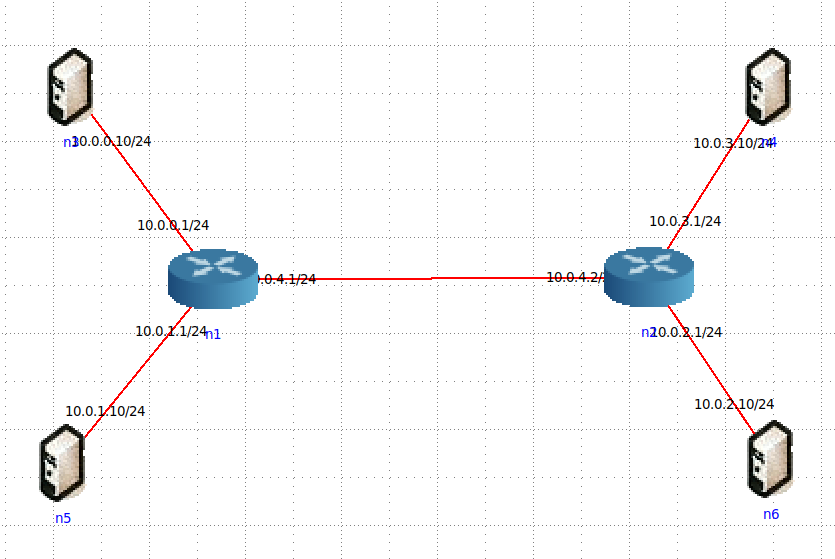
\includegraphics[width=0.5\textwidth]{delay_partition_topology}
	\captionof{figure}{`Partition' network topology.}
	\label{fig:partition_topology}
\end{minipage}

\begin{figure}[H]
\centering
\begin{subfigure}{.5\textwidth}
  \centering
  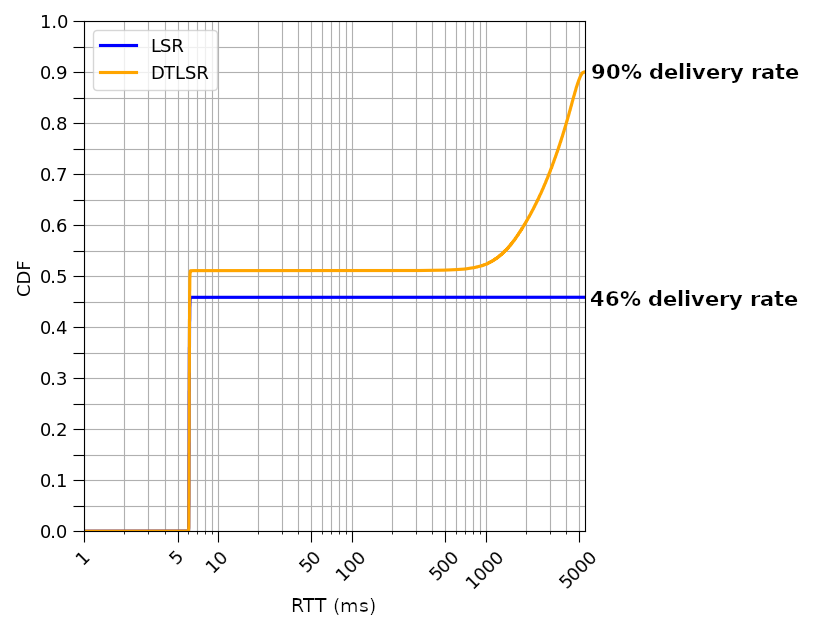
\includegraphics[width=1\linewidth]{delay_partition_flap5}
  \caption{Flapping with period $T=\SI{10}{\s}$ (\SI{5}{\s} up, \SI{5}{\s} down).}
  \label{fig:partition_5}
\end{subfigure}%
\begin{subfigure}{.5\textwidth}
  \centering
  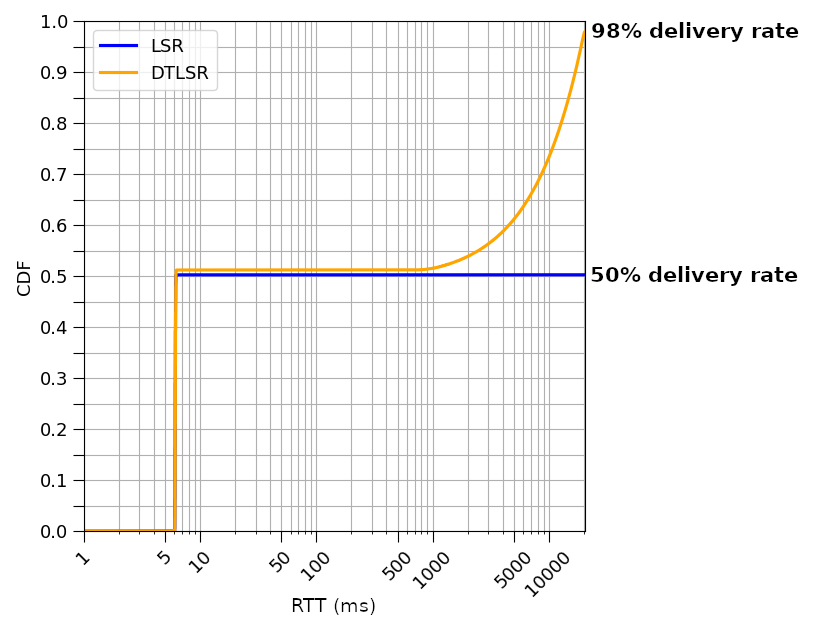
\includegraphics[width=1\linewidth]{delay_partition_flap20}
  \caption{Flapping with period $T=\SI{40}{\s}$ (\SI{20}{\s} up, \SI{20}{\s} down).}
  \label{fig:partition_20}
\end{subfigure}
\caption{Cumulative distributions of end-to-end delay between \texttt{n5} and \texttt{n6} under different routing algorithms, while flapping link \texttt{n1-n2}.}
\label{fig:partition}
\end{figure}

We see in both cases that LSR successfully delivers approximately half of the packets, consistent with the fact that the network is partitioned for half of the time. DTLSR achieves a much higher delivery proportion in both cases due to packets being buffered at the router before the failed link, then forwarded on once the link comes back up. We also see that higher frequency flapping creates a higher drop rate overall for both protocols, which can be explained by considering that when a link goes down it takes time for the router to detect this change, in which time any incoming packets are sent out of the interface and are summarily deleted. It is only once the state change is detected that we change our routing tables or start buffering packets, for LSR and DTLSR respectively. The higher the flapping frequency, the higher proportion of time we spend in these `boundary' periods, and thus the more packets we drop for both LSR and DTLSR.

For DTLSR we have the short delay of \SI{6}{\ms} for approximately half of the packets, and for the other half the delay increases linearly (showing as an exponential curve in the $\log x$-$y$ graph). The first half is due to the link being up half of the time, so all packets sent in this period take approximately the same time to arrive. The second half is a little more subtle, and is due to the packet replaying behaviour. \texttt{ping} sends packets at a constant interval but the buffered packets are replayed all at once when the link comes back up, thus the earlier that a ping is sent in the link-down period, the greater time delay there will be between the client sending the packet and receiving a reply.

This variability in delay can be undesirable, but it is not something that can be fixed as partitioning is a fundamental property of the network that we can't work around. Even a perfect retransmission protocol would run into the same variability issue, retransmitting all of the dropped packets as soon as the link came back up. Users of the network should take this into account with the applications that they decide to run on it, and ensure that there are not strict low-latency requirements with applications like video conferencing or real-time games.

This network topology is consistent with those seen in remote regions even in developed countries, where there is a single main link being relied on. If that link becomes unreliable, then we have shown that using a delay-tolerant routing protocol greatly increases the proportion of packets delivered. One could imagine a situation where the link is only up for a small proportion of the total time, instead of half-and-half, in which case DTLSR would show an even greater advantage over LSR.


\subsubsection{Box Topology}

Our second topology is a `box'-shaped one, where we have a low-delay main route and a higher delay backup route when the main one goes down. In this example \texttt{n3-n4} is the main link that we flap, and \texttt{n3-n5-n6-n4} is our higher-delay backup route. Every link has \SI{1}{\ms} of delay. Thus from \texttt{n1} to \texttt{n2}, our main route has a delay of \SI{3}{\ms} and our backup route has a delay of \SI{5}{\ms}.

\begin{minipage}{1\textwidth} \centering
	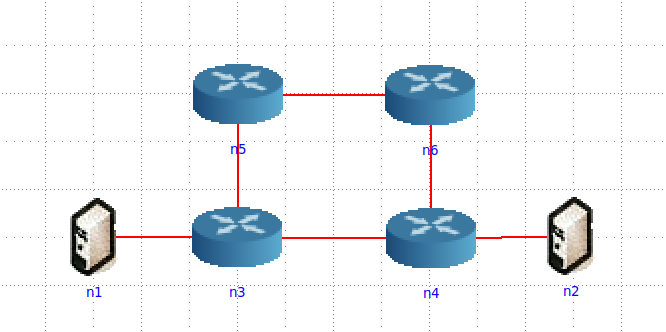
\includegraphics[width=0.5\textwidth]{delay_box_topology}
	\captionof{figure}{`Box' network topology.}
\end{minipage}

\begin{figure}[H]
\centering
\begin{subfigure}{.5\textwidth}
  \centering
  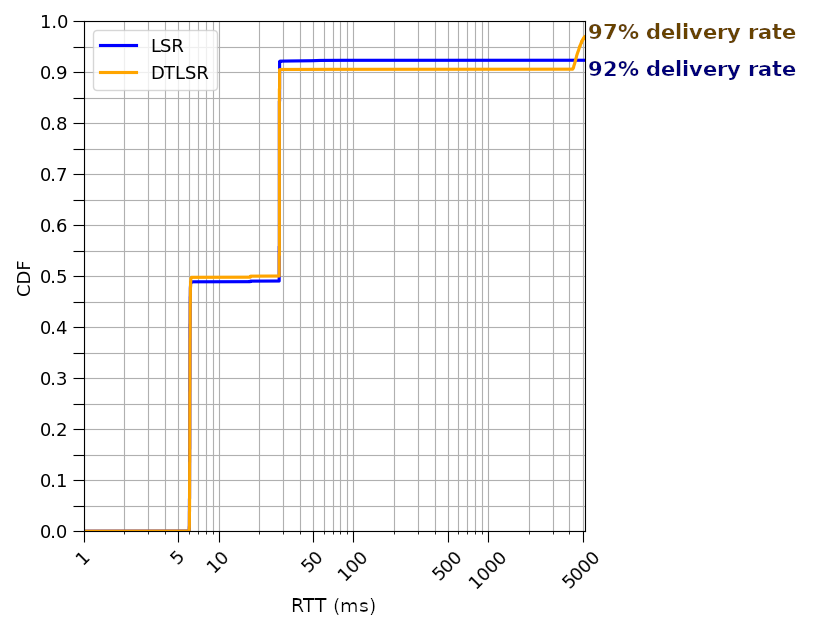
\includegraphics[width=1\linewidth]{delay_box_flap5}
  \caption{Flapping with period $T=\SI{10}{\s}$ (\SI{5}{\s} up, \SI{5}{\s} down).}
  \label{fig:box_5}
\end{subfigure}%
\begin{subfigure}{.5\textwidth}
  \centering
  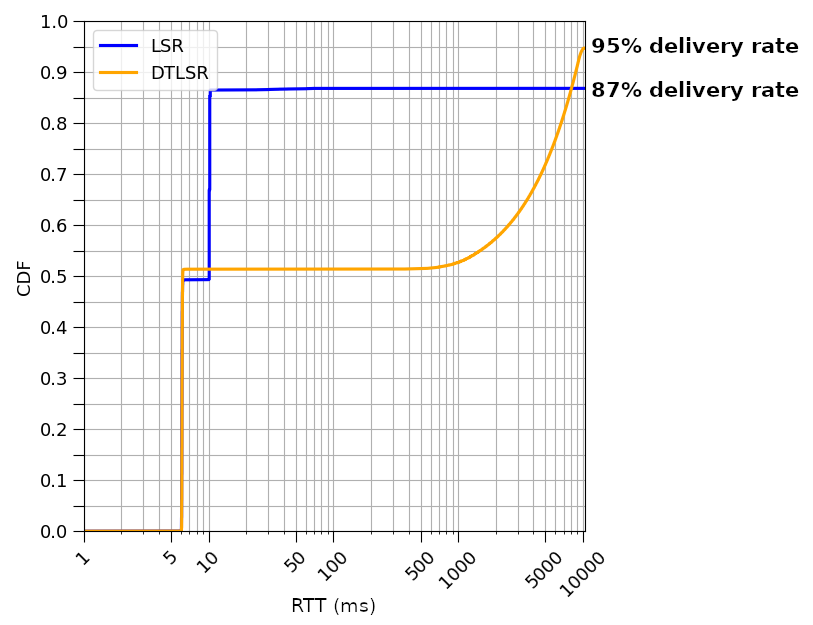
\includegraphics[width=1\linewidth]{delay_box_flap10}
  \caption{Flapping with period $T=\SI{20}{\s}$ (\SI{10}{\s} up, \SI{10}{\s} down).}
  \label{fig:box_20}
\end{subfigure}
\caption{Cumulative distributions of end-to-end delay between \texttt{n1} and \texttt{n2} under different routing algorithms, while flapping link \texttt{n3-n4}.}
\label{fig:box}
\end{figure}

We see in both cases that LSR successfully switches to the backup link whenever the main link goes down, shown by a large proportion of packets having an RTT of approximately \SI{10}{\ms}. As described above, it takes time for the protocol to detect that the link is down and to respond by modifying the routing table, which causes packet losses. Increasing the flapping frequency increases the number of these boundary periods, thus increasing the proportion of time dropping packets. This is reflected in the higher proportion of packets being dropped with a shorter flapping period for LSR.

We again see that DTLSR achieves a higher proportion of delivered packets than LSR. While it is a lot closer than in the partition topology, there is still a marked difference. DTLSR does not choose to switch to the backup link, and instead continues buffering packets waiting for the main link to come back up. It is interesting to compare LSR and DTLSR in these periods where the main link is down. LSR achieves a much lower delay than DTLSR by switching to the backup link, but DTLSR delivers those packets much more reliably. The choice here likely depends on what applications the user wants to run over the network. For applications with strict low-latency requirements like video conferencing software, LSR is likely better, but for applications that want reliable transfer with minimal retransmissions like bulk file transfers, DTLSR is the better choice.

As stated above this kind of topology is uncommon in remote and developing regions due to the cost of adding backup links. However it is useful to contrast LSR and DTLSR in other environments to see fully their strengths and weaknesses.


\subsubsection{Full Partition Topology}

Our third topology is similar to the above `partition' topology, but instead partitions the network with two links in sequence that have anti-correlated failures (When one is up, the other is down). Thus there is never any end-to-end connection and the network is technically always partitioned, but using the `store-and-forward' mechanism some packet delivery can be achieved. This is not as ridiculous a case as it may seem. If a region has unreliable or limited power, there may only be power to turn on a subset of the routers at a time, likely in an unpredictable pattern.

\begin{figure}[H]
\centering
\begin{subfigure}{.5\textwidth}
  \centering
  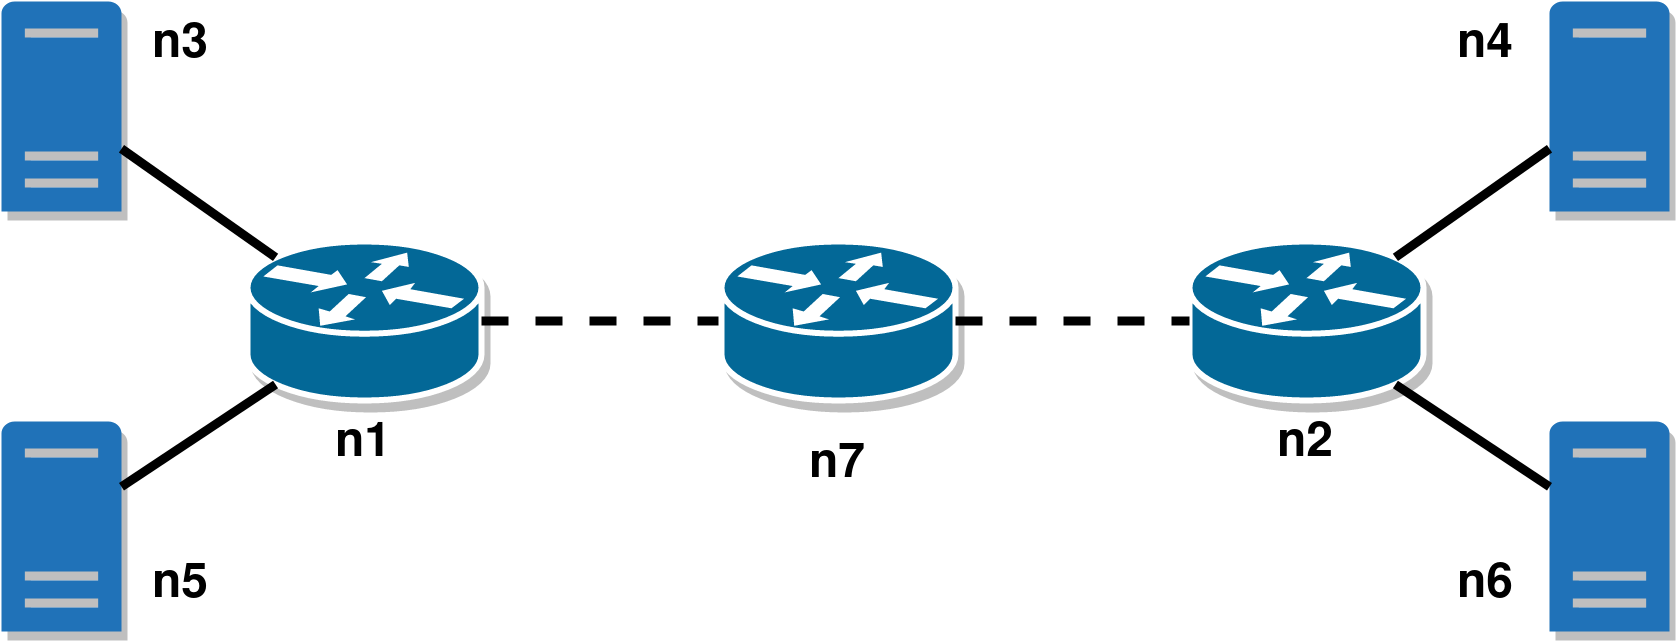
\includegraphics[width=1\linewidth]{delay_full_partition_topology}
  \label{fig:full_partition_topology}
\end{subfigure}%
\begin{subfigure}{.5\textwidth}
  \centering
  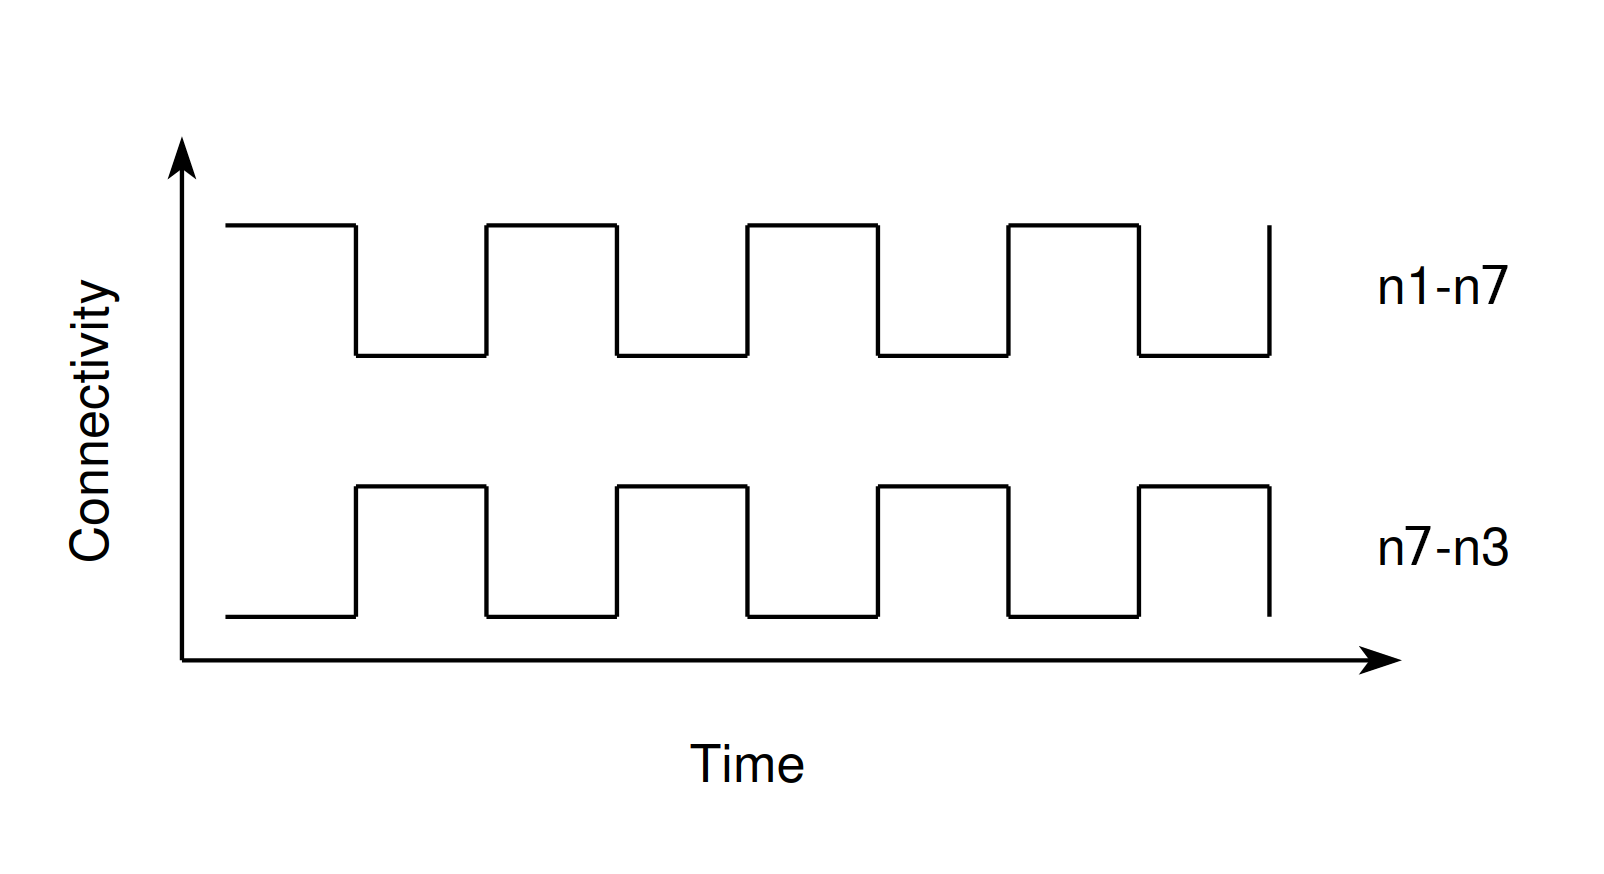
\includegraphics[width=1\linewidth]{delay_full_partition_graph}
  \label{fig:full_partition_graph}
\end{subfigure}
\caption{`Full partition' network topology with anti-correlated failures.}
\label{fig:full_partition}
\end{figure}

\begin{minipage}{1\textwidth} \centering
	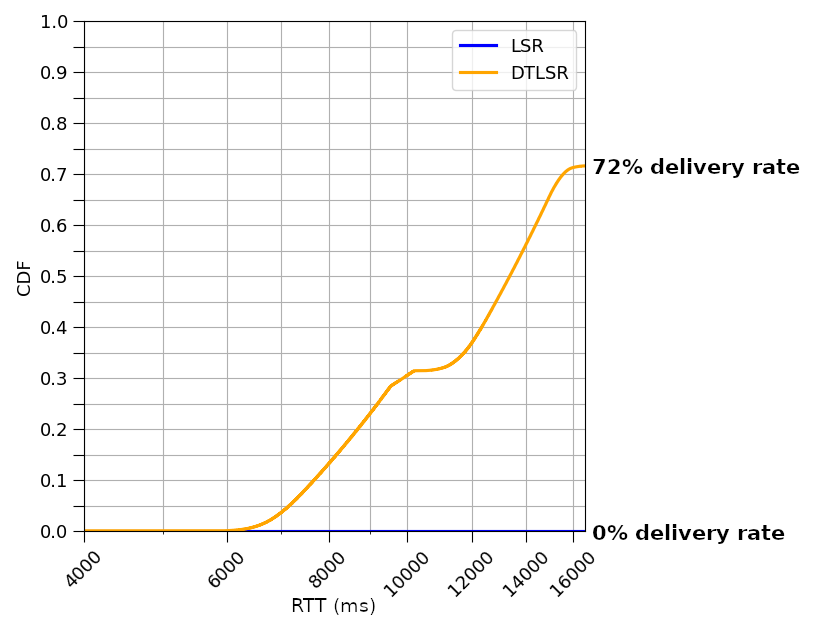
\includegraphics[width=0.75\textwidth]{delay_full_partition_flap5}
	\captionof{figure}{Flapping with period $T=\SI{10}{\s}$ (\SI{5}{\s} up, \SI{5}{\s} down).}
\end{minipage}

We see that LSR achieves zero packet delivery, compared to DTLSR achieving x percent overall. This is notably much more serious than the results above, where LSR achieved a lower but still greater-than-zero delivery, as retransmission-based transport protocols rely on the fact that there is \textit{some} packet delivery, where in the limit of time with retransmissions the probability of delivery approaches 1. However with zero delivery, this limit stays at zero and thus our unreliable network cannot be made reliable with a transport layer protocol. We rely entirely on the routing layer's buffering to achieve any communication whatsoever.

\subsubsection{TCP}

TCP fundamentally does not work well in a variable-delay environment. It works best when the estimated RTT is close to the real delay; in the case where the delay suddenly increases (e.g. a link failure), there will be a long string of packet timeouts in quick succession, dropping the sending window to its minimum size due to the multiplicative decrease (AIMD). Even if these packets have been buffered up before the failure as in DTLSR, the sending node will retransmit them, wasting network resources. If the failure is longer-term, we may retransmit multiple times, ending up buffering many identical copies of the packet before the link failure. This has a great risk of overflowing the buffer with redundant data.


\section{Conclusions}

\section{Bibliography}

\section{Appendices}

\section{Index}

\section{Project Proposal}



\end{document}





























